\chapter{Application for local damage detection}\label{chap:application}
\section{Application for simulated data}
\subsection{Cyclic sources extraction from complex multiple-component vibration signal via periodically time varying filter}
Firstly, the methodology introduced in Section~\ref{sec:chapter7/semi_blind/schemat_przekladniasemi_blind_methodology} is applied to the simulated data. Such application gives a possibility to check if the algorithm performs appropriately for the entirely known signal. We would like to analyzed three cases. In particular, first one consists of two different components corresponded to the fault. In order to test the performance in case of variable period of the damage the signal with jitter is simulated. Finally, in the last case the signal without any cyclic component is analyzed with proposed method. It would inform how the proposed method is sensitive for the false alarm.

\subsubsection{Signal with multiple fault source}
\label{sec:chapter7/semi_blind/schemat_przekladniamultiple source_semi_blind}
Let us analyse firstly the signal with multiple cyclic components. It corresponds to the machine, in which two damages occur. One can be interested if the method is able to extract both cyclic components.
The length of the signal is 2.5 seconds and the sampling frequency is  8192~Hz. The signal is presented in time and time-frequency domain in Fig.~\ref{fig:chapter7/semi_blind/time-plot_sim}.
\begin{figure}[!ht]
    \centering
    \begin{subfigure}[b]{0.8\textwidth}
        \centering
        \captionsetup{skip=0.01pt}
         \caption{}
        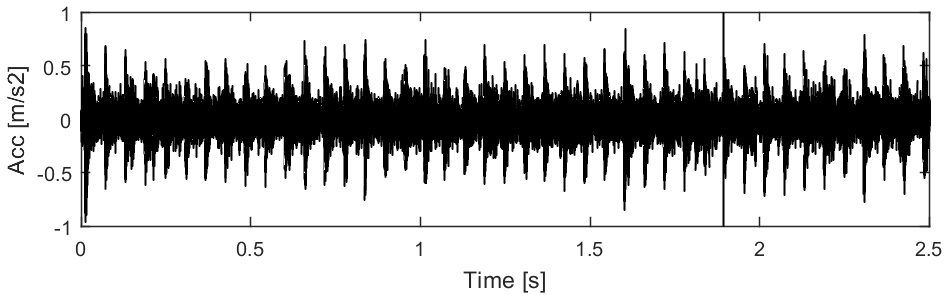
\includegraphics[width=\textwidth]{wykresy/chapter_application/semi_blind/sygnal_simulated.png}
        % \label{fig:chapter7/semi_blind/time_sim}
    \end{subfigure}
    %\hfill
    \begin{subfigure}[b]{0.7\textwidth}
        \centering
        \captionsetup{skip=0.01pt}
         \caption{}
        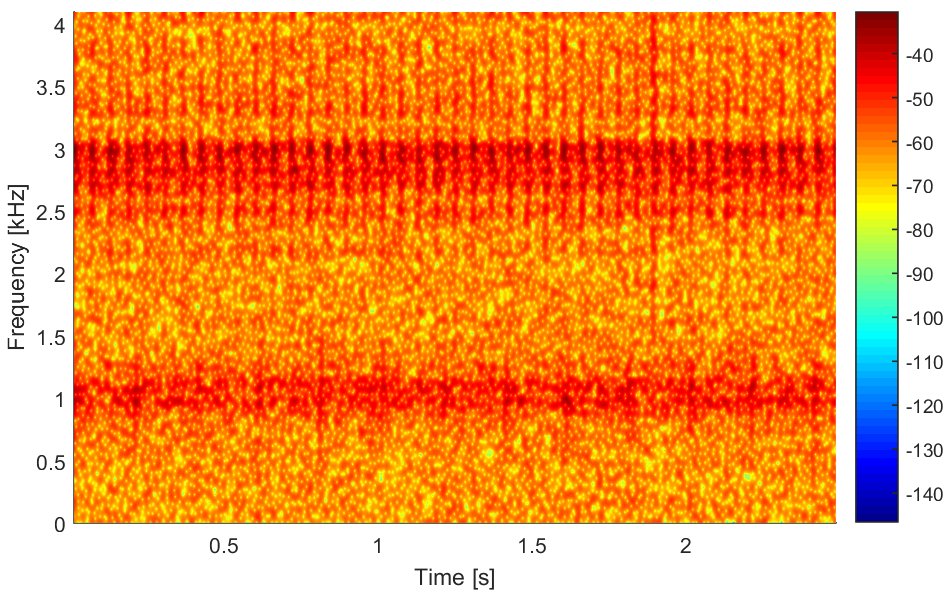
\includegraphics[width=\textwidth]{wykresy/chapter_application/semi_blind/spectrogram_simulated.png}
        % \label{fig:chapter7/semi_blind/spectrogram_sim}
    \end{subfigure}
%    \hfill
    \begin{subfigure}[b]{0.8\textwidth}
        \centering
        \captionsetup{skip=0.01pt}
        \caption{}
        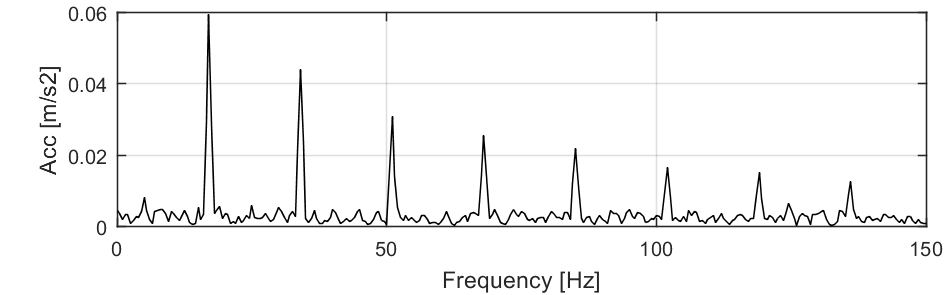
\includegraphics[width=\textwidth]{wykresy/chapter_application/semi_blind/widmo_obwiedni_simulated.png}
        \label{fig:chapter7/semi_blind/obwiednia_sim}
    \end{subfigure}
    \caption{Time plot (a), spectrogram (b) and envelope spectrum (c) of the vibration simulated signal with two damages. The spectrogram parameters are as follows: $N_w=250$, $Ov=96\%$.}
    \label{fig:chapter7/semi_blind/time-plot_sim}
\end{figure}
\\
There are two periodic impulse trains with modulation frequencies 5~Hz and 17~Hz, respectively, and random noise added to each pulse train. Corresponding time plots are presented in Fig.~\ref{fig:chapter7/semi_blind/sim_skladowe}, where periodic impulses can be observed. These components represent local fault, which can occur in a rotating machine. The carrier frequency bands are 700-1300~Hz and 2300-3200~Hz for modulation frequencies 5~Hz and 17~Hz, respectively. The former amplitudes have values around $\pm 0.02$ and the later one are approximately $\pm 0.04$. For both components the white noise with amplitudes $\pm 0.01$ was added. The spectrogram parameters are as follows: $N_w=250$, $Ov=96\%$. According to envelope spectrum (Fig.~\ref{fig:chapter7/semi_blind/obwiednia_sim}) of the raw simulated signal only harmonics for 17~Hz can be observed. The amplitude of impulses with modulation frequency 5~Hz is significantly lower, thus corresponding harmonics are hidden.
\begin{figure}[!ht]
    \centering
    \begin{subfigure}[b]{0.9\textwidth}
        \centering
        \captionsetup{skip=0.01pt}
         \caption{}
        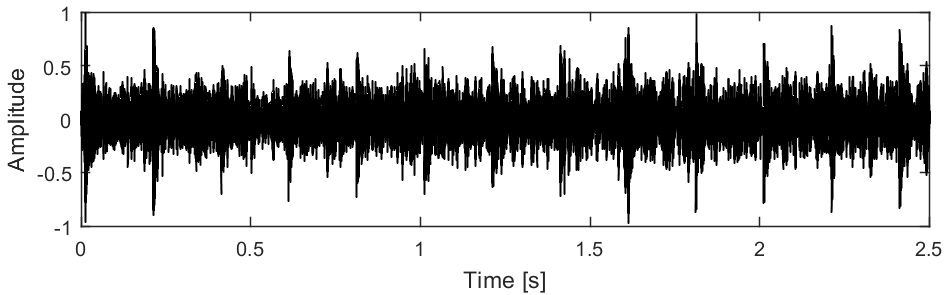
\includegraphics[width=\textwidth]{wykresy/chapter_application/semi_blind/sygnal_ff5_simulated.png}
        % \label{fig:chapter7/semi_blind/time_sim_skladowa5}
    \end{subfigure}
    %\hfill
    \begin{subfigure}[b]{0.9\textwidth}
        \centering
        \captionsetup{skip=0.01pt}
         \caption{}
        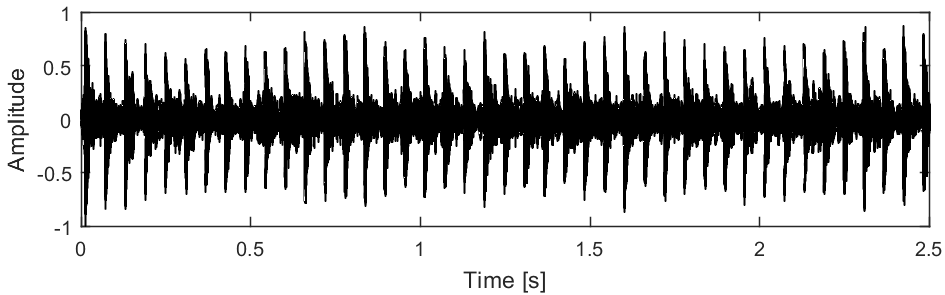
\includegraphics[width=\textwidth]{wykresy/chapter_application/semi_blind/sygnal_ff17_simulated.png}
        % \label{fig:chapter7/semi_blind/time_sim_skladowa17}
    \end{subfigure}
    \caption{Time plots of the normalized impulse trains with modulation frequencies 5~Hz (a) and 17~Hz (b).}
    \label{fig:chapter7/semi_blind/sim_skladowe}
\end{figure}
%
\begin{figure}[!ht]
    \centering
    \begin{subfigure}[b]{0.49\textwidth}
        \centering
        \captionsetup{skip=0.01pt}
        \caption{}
        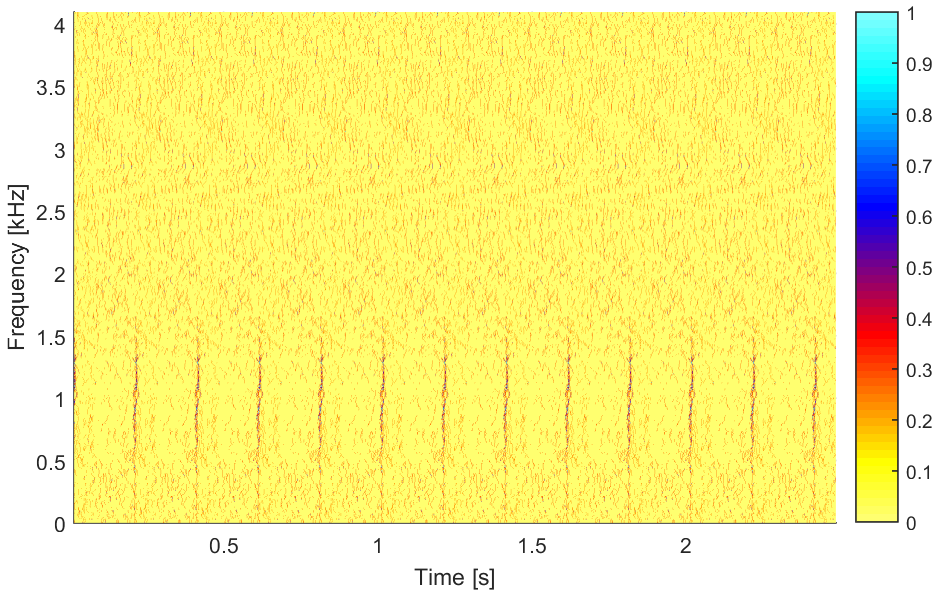
\includegraphics[width=\textwidth]{wykresy/chapter_application/semi_blind/wagi_simulated_5.png}
        \label{fig:chapter7/semi_blind/wagi_sim_5}
    \end{subfigure}
\vspace{-1\baselineskip}
    \begin{subfigure}[b]{0.49\textwidth}
        \centering
        \captionsetup{skip=0.01pt}
        \caption{}
        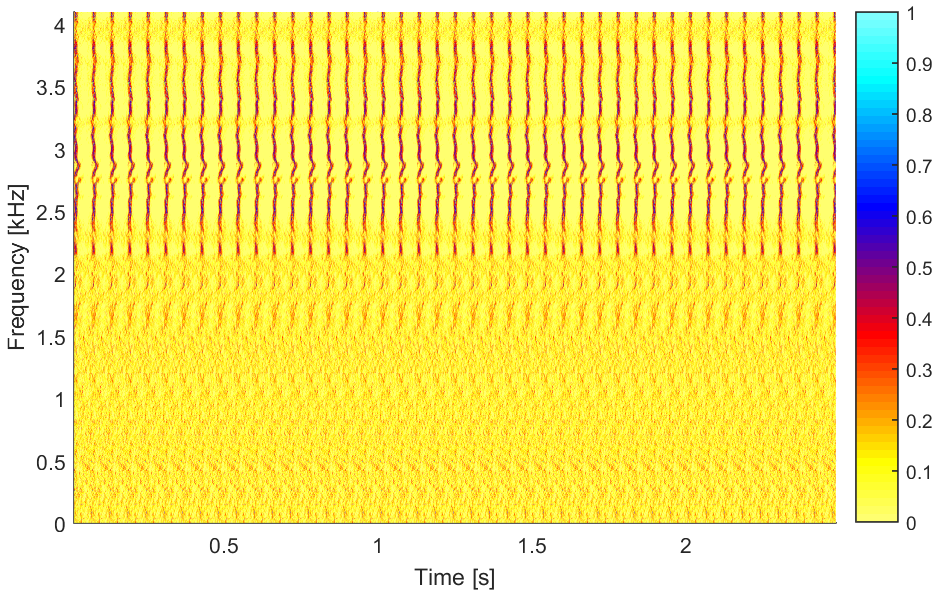
\includegraphics[width=\textwidth]{wykresy/chapter_application/semi_blind/wagi_simulated_17.png}
        \label{fig:chapter7/semi_blind/wagi_sim_17}
    \end{subfigure}
\vspace{-1\baselineskip} 
    \begin{subfigure}[b]{0.49\textwidth}
        \centering
        \captionsetup{skip=0.01pt}
        \caption{}
        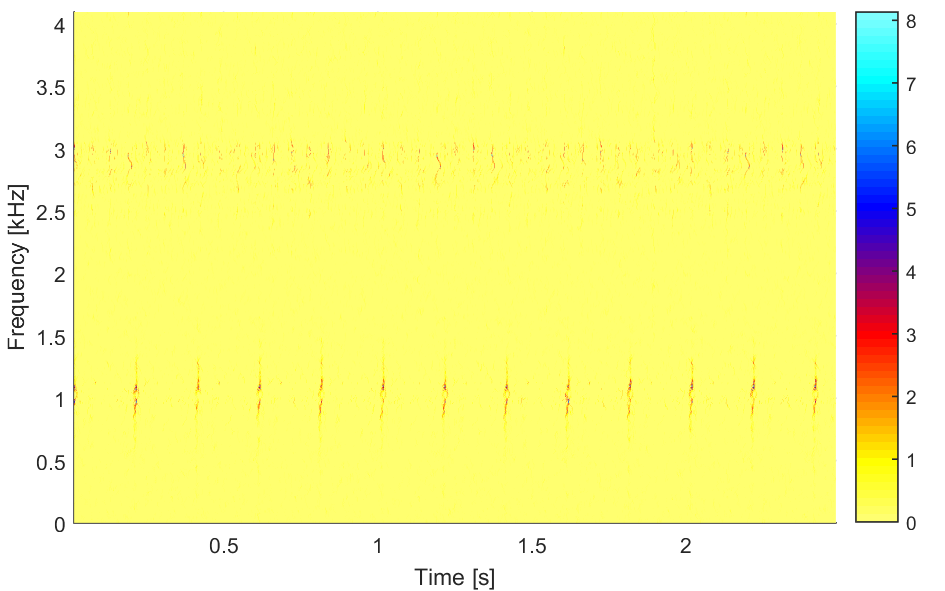
\includegraphics[width=\textwidth]{wykresy/chapter_application/semi_blind/mapka_simulated_5.png}
        \label{fig:chapter7/semi_blind/mapka_sim_5}
    \end{subfigure}
    %\hfill
    \begin{subfigure}[b]{0.49\textwidth}
        \centering
        \captionsetup{skip=0.01pt}
        \caption{}
        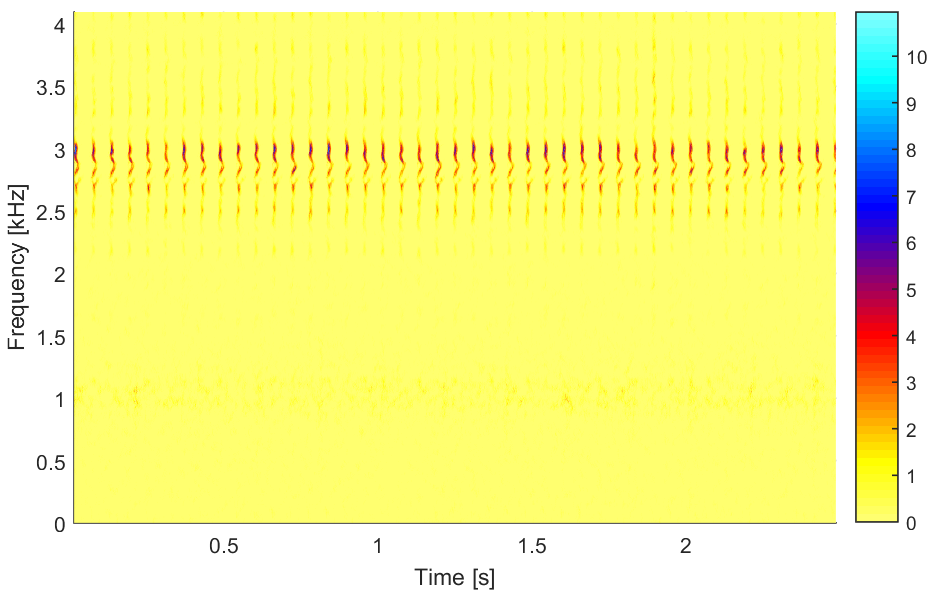
\includegraphics[width=\textwidth]{wykresy/chapter_application/semi_blind/mapka_simulated_17.png}
        \label{fig:chapter7/semi_blind/mapka_sim_17}
    \end{subfigure}
    \vspace{\baselineskip}
    \caption{Score matrices for fault frequency 5~Hz (a) and fault frequency 17~Hz (b). The weighted spectrogram (time-varying filter coefficients) for fault frequency 5~Hz (c) and fault frequency 17~Hz (d). }
    \label{fig:chapter7/semi_blind/score_sim}
\end{figure} \\
In this study we applied the proposed source separation algorithm for two different fault frequencies in order to illustrate its basic properties. Due to spectrogram parameters, the range $r$ corresponding to fault frequency 5~Hz is equal to 164. Binary maps $M$ for both cyclic frequencies are calculated and score maps are derived upon them. The score maps are presented in Figs.~\ref{fig:chapter7/semi_blind/wagi_sim_5} and~\ref{fig:chapter7/semi_blind/wagi_sim_17}. One can notice some noise in these maps, i.e. above 1500~Hz and below 2000~Hz for 5~Hz and 17~Hz cyclic frequencies, respectively. This noise is not related to the periodic amplitude modulation, since there are no clearly visible lines along the frequency axis in these frequency bands. Time-varying filter coefficients are represented by two-dimensional maps in Figs.~\ref{fig:chapter7/semi_blind/mapka_sim_5} and~\ref{fig:chapter7/semi_blind/mapka_sim_17}. Recall that these are raw spectrograms multiplied element-wise by score maps. One can notice that the random noise in score maps does not influence the filter characteristics. Non-zero scores not related to periodic modulations result in low filter coefficient, while multiplied by the spectrogram value. On the other hand, high values of the score map are related to periodic modulation and multiplication by the spectrogram values results in a high value of the time-varying filter coefficients. According to the results, the novel algorithm automatically indicates points in the spectrograms related to given fault frequencies.\\
Given two weighted spectrograms the inverse short-time Fourier transform might be applied in order to return to the time domain. In case of the simulated signal, there is a possibility to compare the raw components and the extracted time series representing sources. The comparison is presented in Fig.~\ref{fig:chapter7/semi_blind/comp_comparison_sim}. Clearly, the extracted signal components are similar to simulated. The impulses reveal in the same time points, with similar amplitudes of corresponding impulses. Moreover, the noise level is lower for extracted components, thus the impulses are even more visible. Noise level in Fig.~\ref{fig:chapter7/semi_blind/syg_comp5_sim} is about 0.3 while in the extracted signal it is close to 0.2. In case of 17~Hz amplitude modulation the noise level is close to 0.2 and 0.1 for raw and extracted signal, respectively. Presented results for the simulated data sample confirm that the proposed methodology can be applied for cyclic source extraction from the raw signal that consists of two pulse trains, each with different carrier and cyclic frequencies. In Fig.~\ref{fig:chapter7/semi_blind/widmo_comp_comparison_sim} the envelope spectra for each analyzed signal component and the corresponding extracted source signals are provided. One can observe that in both cases several harmonics related to fault frequencies are indicated. This confirms that the extracted signals follow the cyclic modulation from the raw signals. It is wort mentioning that in the raw signals only the harmonics corresponding to cyclic frequency 17~Hz were detected. (Fig.~\ref{fig:chapter7/semi_blind/obwiednia_sim}).
\begin{figure}[!ht]
    \centering
    \begin{subfigure}[b]{0.49\textwidth}
        \centering
        \captionsetup{skip=0.01pt}
        \caption{}
        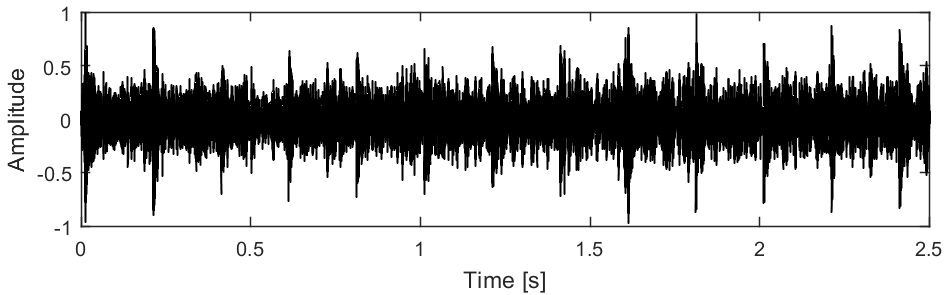
\includegraphics[width=\textwidth]{wykresy/chapter_application/semi_blind/sygnal_ff5_simulated.png}
        \label{fig:chapter7/semi_blind/syg_comp5_sim}
    \end{subfigure}
    \vspace{-1\baselineskip}
    \begin{subfigure}[b]{0.49\textwidth}
        \centering
        \captionsetup{skip=0.01pt}
        \caption{}
        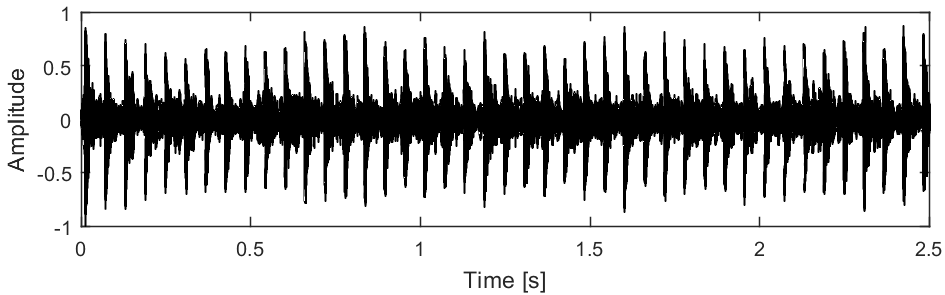
\includegraphics[width=\textwidth]{wykresy/chapter_application/semi_blind/sygnal_ff17_simulated.png}
        \label{fig:chapter7/semi_blind/syg_comp17_sim}
    \end{subfigure}
    \vspace{-1\baselineskip}  
    \begin{subfigure}[b]{0.49\textwidth}
        \centering
        \captionsetup{skip=0.01pt}
        \caption{}
        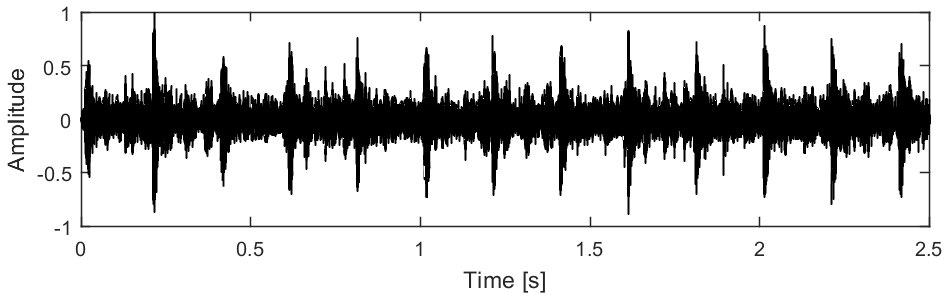
\includegraphics[width=\textwidth]{wykresy/chapter_application/semi_blind/sygnal_simulated_5.png}
        \label{fig:chapter7/semi_blind/ext_comp5_sim}
    \end{subfigure}
    %\hfill
    \begin{subfigure}[b]{0.49\textwidth}
        \centering
        \captionsetup{skip=0.01pt}
        \caption{}
        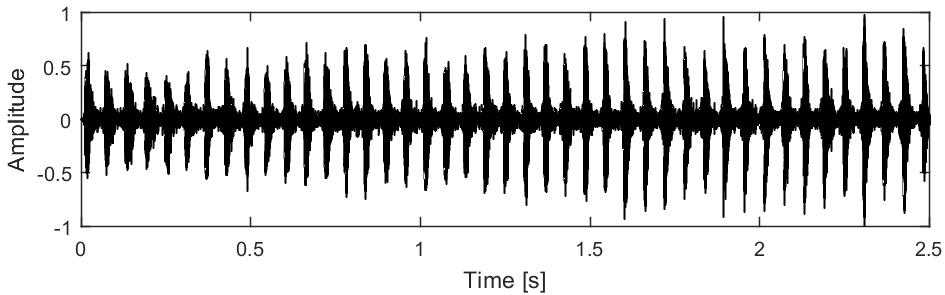
\includegraphics[width=\textwidth]{wykresy/chapter_application/semi_blind/sygnal_simulated_17.png}
        \label{fig:chapter7/semi_blind/ext_comp17_sim}
    \end{subfigure}
    \vspace{\baselineskip}
    \caption{The normalized components of the simulated signal with modulation frequency 5~Hz (a) and 17~Hz (b). The normalized extracted signal from weighted spectrogram for fault frequency 5~Hz (c) and 17~Hz(d). }
    \label{fig:chapter7/semi_blind/comp_comparison_sim}
\end{figure}
%
\begin{figure}[!ht]
    \centering
    \begin{subfigure}[b]{0.49\textwidth}
        \centering
        \captionsetup{skip=0.01pt}
        \caption{}
        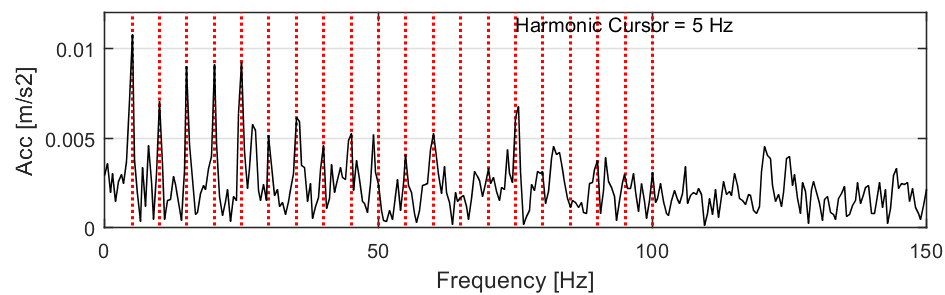
\includegraphics[width=\textwidth]{wykresy/chapter_application/semi_blind/widmo_obwiedni_simulated_comp5.png}
    \end{subfigure}
    % \vspace{-1\baselineskip}
    \begin{subfigure}[b]{0.49\textwidth}
        \centering
        \captionsetup{skip=0.01pt}
        \caption{}
    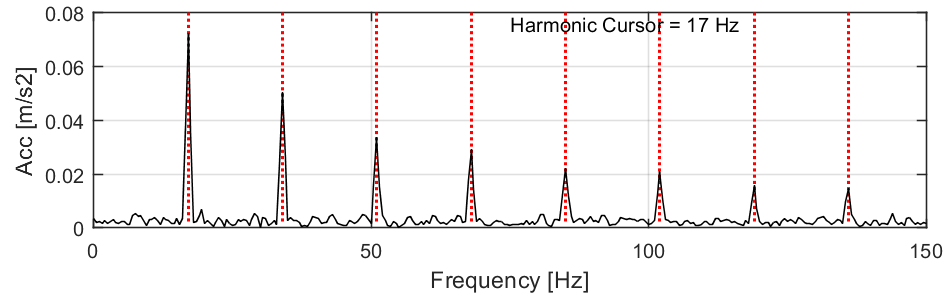
\includegraphics[width=\textwidth]{wykresy/chapter_application/semi_blind/widmo_obwiedni_simulated_comp17.png}
    \end{subfigure}
    % \vspace{-1\baselineskip}  
    \begin{subfigure}[b]{0.49\textwidth}
        \centering
        \captionsetup{skip=0.01pt}
        \caption{}
        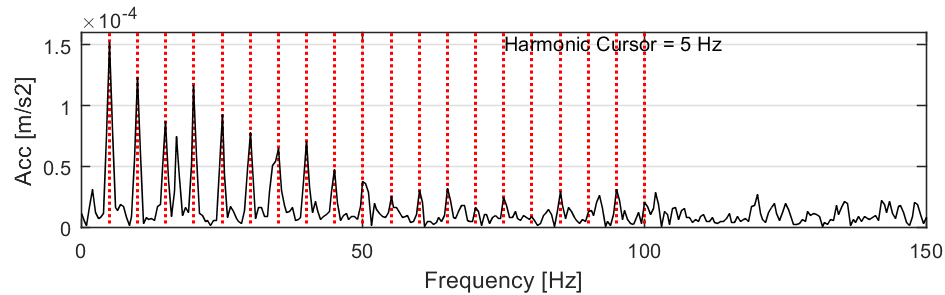
\includegraphics[width=\textwidth]{wykresy/chapter_application/semi_blind/widmo_obwiedni_simulated_5.png}
    \end{subfigure}
    %\hfill
    \begin{subfigure}[b]{0.49\textwidth}
        \centering
        \captionsetup{skip=0.01pt}
        \caption{}
        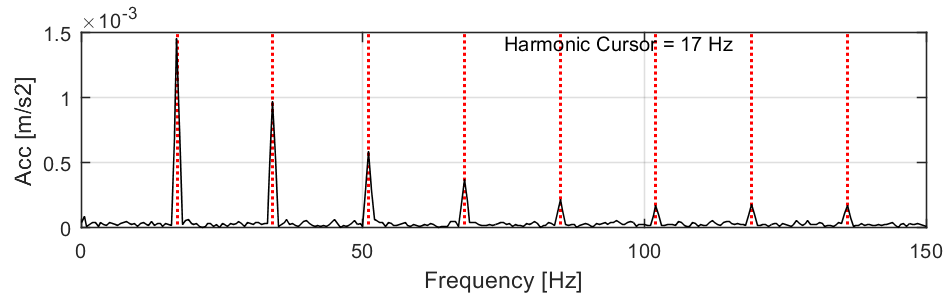
\includegraphics[width=\textwidth]{wykresy/chapter_application/semi_blind/widmo_obwiedni_simulated_17.png}
        
    \end{subfigure}
    \vspace{\baselineskip}
    \caption{The envelope spectrum of the simulated signal with modulation frequency 5~Hz (a) and 17~Hz (b). The extracted signal envelope spectrum from weighted spectrogram for fault frequency 5~Hz (c) and 17~Hz(d). }
    \label{fig:chapter7/semi_blind/widmo_comp_comparison_sim}
\end{figure}
\subsection{Signal representing bearing jitter effect}
One can be interested how the proposed method is performing in case of small variation of fault frequency. In particular, we would like to analyze the signal in which the period of the fault occurrence is not constant. Therefore, the signal, which resemble the bearing with jitter is simulated. The rotational speed is equal to 1.3 Hz and the sampling frequency is 8192~Hz. One cyclic pulse train with modulation frequency 5~Hz is added and it has a jitter effect. The carrier frequency bands are 700-1300~Hz. The amplitude of the impulses are around 1. Furthermore, the Gaussian random noise with mean 0 and standard deviation $4/3$. The waveform of the signal is presented in Fig. \ref{fig:chapter7/semi_blind/time_jitter}. 
\begin{figure}[!ht]
    \centering
    \begin{subfigure}[b]{0.8\textwidth}
        \centering
        \captionsetup{skip=0.01pt}
         \caption{}
        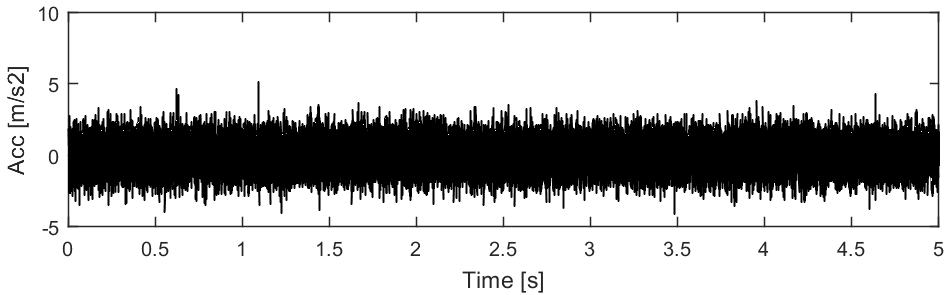
\includegraphics[width=\textwidth]{wykresy/chapter_application/semi_blind/sygnal_jitter.png}
        \label{fig:chapter7/semi_blind/time_jitter}
    \end{subfigure}
    %\hfill
    \begin{subfigure}[b]{0.7\textwidth}
        \centering
        \captionsetup{skip=0.01pt}
         \caption{}
        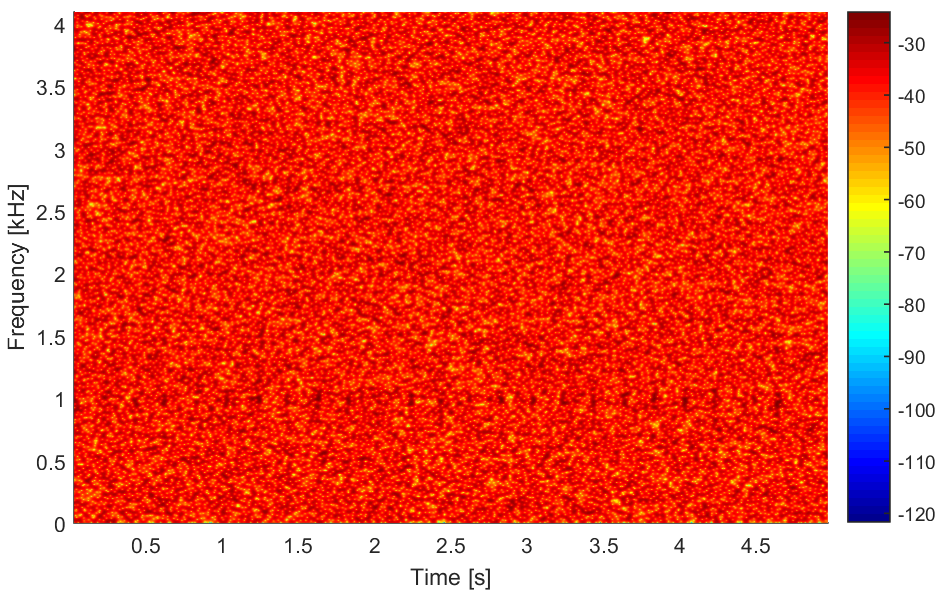
\includegraphics[width=\textwidth]{wykresy/chapter_application/semi_blind/spectrogram_jitter.png}
        \label{fig:chapter7/semi_blind/spectrogram_jitter}
    \end{subfigure}
%    \hfill
    \begin{subfigure}[b]{0.8\textwidth}
        \centering
        \captionsetup{skip=0.01pt}
        \caption{}
        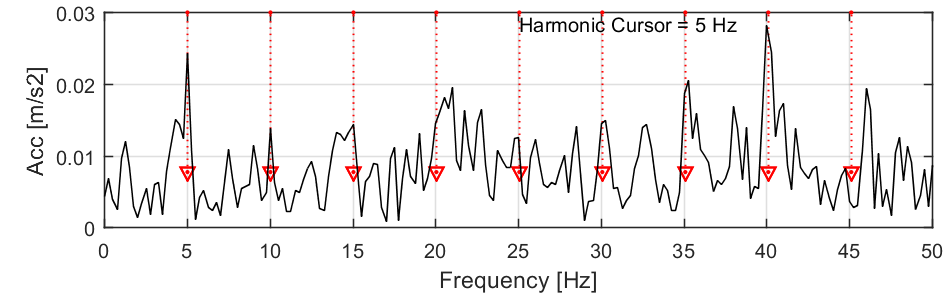
\includegraphics[width=\textwidth]{wykresy/chapter_application/semi_blind/widmo_obwiedni_jitter.png}
        \label{fig:chapter7/semi_blind/obwiednia_jitter}
    \end{subfigure}
    \caption{Time plot (a), spectrogram (b) and envelope spectrum (c) of the vibration simulated signal with bearing jitter effect. The spectrogram parameters are as follows: $N_w=250$, $Ov=96\%$.}
\end{figure}
The impulses are barely visible on the time-frequency map (Fig. \ref{fig:chapter7/semi_blind/spectrogram_jitter}). Furthermore, on the envelope spectrum the harmonics correspond to fault frequency cannot be observed (Fig. \ref{fig:chapter7/semi_blind/obwiednia_jitter}). Thus, it is a complicated signal with invisible fault component, where the standard envelope methods for fault detection fail. Therefore, we would like to apply proposed method for cyclic source extraction. The extracted cyclic normalized signal component is presented in Fig. \ref{fig:chapter7/semi_blind/time_jitter_filtr}. One can observe that the level of noise is smaller and the impulses are clearly detectable. As it was expected on the envelope spectrum the harmonics related to the fault frequency are observed, namely 7 harmonics are visible. It is shown that the proposed algorithm is performing well in case of the signal with slightly varying fault frequency. Obviously, the results depend on the level of fault frequency variances. However, in case of the reasonable changes of the period of fault occurrence the method is able to extract the signal component related to the fault.
%
\begin{figure}[!ht]
    \centering
    \begin{subfigure}[b]{0.8\textwidth}
        \centering
        \captionsetup{skip=0.01pt}
         \caption{}
        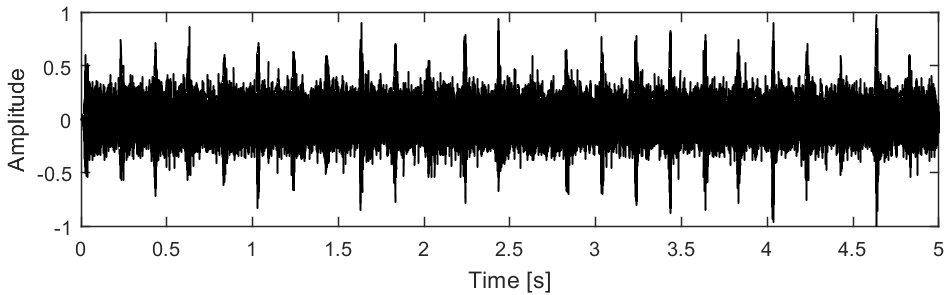
\includegraphics[width=\textwidth]{wykresy/chapter_application/semi_blind/sygnal_jitter_filtr.png}
        \label{fig:chapter7/semi_blind/time_jitter_filtr}
    \end{subfigure}

    \begin{subfigure}[b]{0.8\textwidth}
        \centering
        \captionsetup{skip=0.01pt}
        \caption{}
        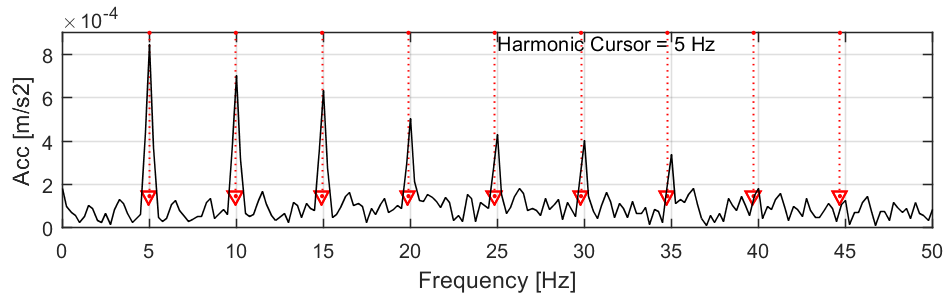
\includegraphics[width=\textwidth]{wykresy/chapter_application/semi_blind/widmo_obwiedni_jitter_filtr.png}
        \label{fig:chapter7/semi_blind/obwiednia_jitter_filtr}
    \end{subfigure}
    \caption{Time plot (a) and envelope spectrum (b) of the extracted cyclic normalized signal component with bearing jitter effect.}
\end{figure}
%
\subsection{Signal without cyclic component}
Finally, we would like to test the performance of the method for the healthy signal. Indeed, the signal without any cyclic component is simulated. The length is equal to 2.5 seconds and the sampling frequency is 8192~Hz. The signal consists of background Gaussian random noise with mean zero and variance equal to 0.2. Furthermore, in the carrier frequency bands 700-1300~Hz and 2300-3200~Hz additional random noise with mean zero and variance  0.2 is added. Therefore, it is signal like in section \ref{sec:chapter7/semi_blind/schemat_przekladniamultiple source} with amplitude of impulses equals to 0. In the analysis the proposed cyclic source extraction method was tested for the modulation frequency 17~Hz. It is expected that as a result, the signal without fault pattern is obtained. It would ensure that the proposed method do not create the cyclic impulses. In Fig. \ref{fig:chapter7/semi_blind/time_zdrowy} the signal without cyclic component is presented. Furthermore, the spectrogram is shown in Fig. \ref{fig:chapter7/semi_blind/spectrogram_zdrowy}, where no impulses are visible. In the envelope spectrum no harmonics of modulation frequency 17~Hz are observed. 
\begin{figure}[!ht]
    \centering
    \begin{subfigure}[b]{0.8\textwidth}
        \centering
        \captionsetup{skip=0.01pt}
         \caption{}
        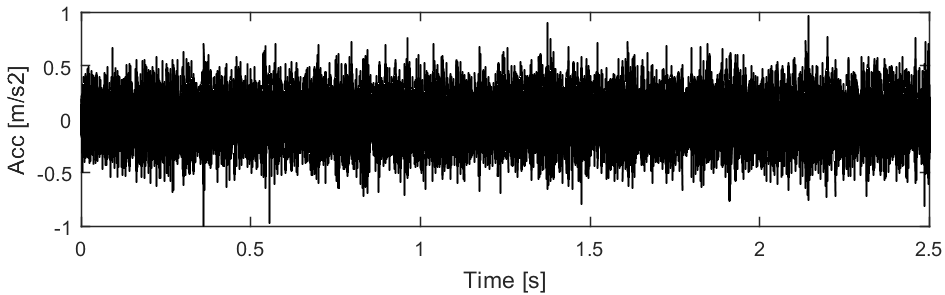
\includegraphics[width=\textwidth]{wykresy/chapter_application/semi_blind/sygnal_bez_impulsow.png}
        \label{fig:chapter7/semi_blind/time_zdrowy}
    \end{subfigure}
    %\hfill
    \begin{subfigure}[b]{0.7\textwidth}
        \centering
        \captionsetup{skip=0.01pt}
         \caption{}
        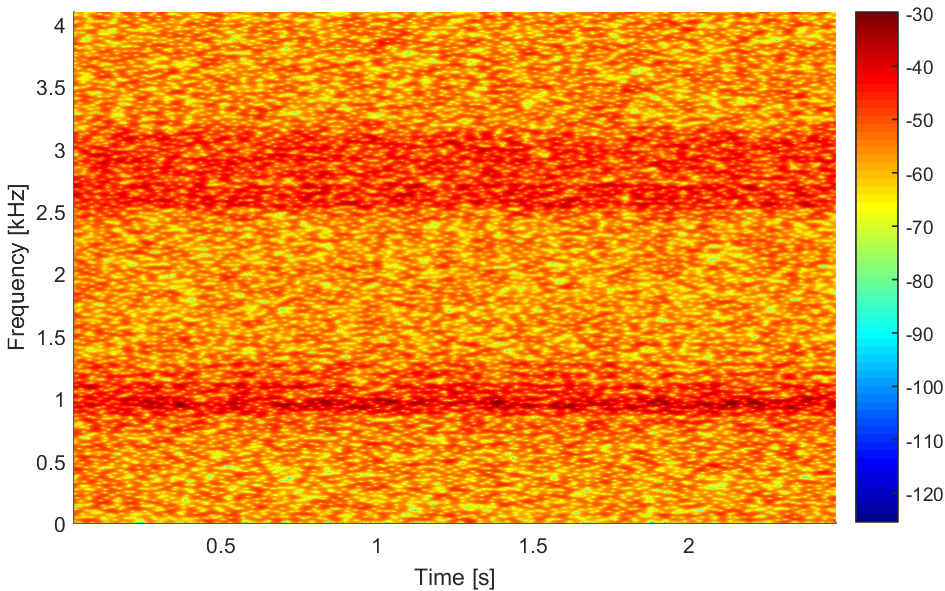
\includegraphics[width=\textwidth]{wykresy/chapter_application/semi_blind/spectrogramsygnal_bez_impulsow.png}
        \label{fig:chapter7/semi_blind/spectrogram_zdrowy}
    \end{subfigure}
%    \hfill
    \begin{subfigure}[b]{0.8\textwidth}
        \centering
        \captionsetup{skip=0.01pt}
        \caption{}
        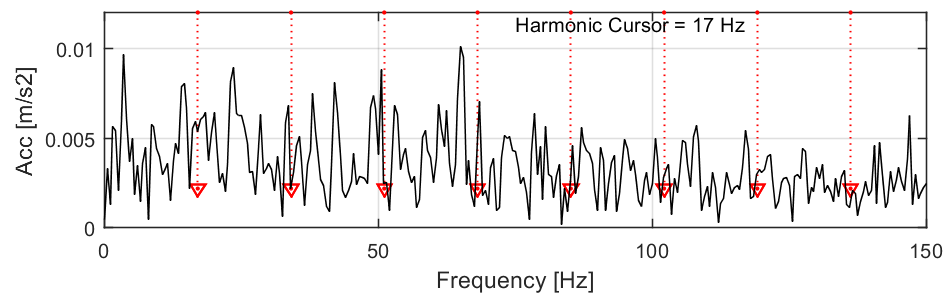
\includegraphics[width=\textwidth]{wykresy/chapter_application/semi_blind/widmo_obwiedni_sygnal_bez_impulsow.png}
        \label{fig:chapter7/semi_blind/obwiednia_zdrowy}
    \end{subfigure}
    \caption{Time plot (a), spectrogram (b) and envelope spectrum (c) of the vibration simulated signal without the fault component. The spectrogram parameters are as follows: $N_w=250$, $Ov=96\%$.}
    \end{figure}
%
The signal after source extraction method application is presented in Fig. \ref{fig:chapter7/semi_blind/time_zdrowy_filtr}. One can observe that it is similar to signal before the processing (Fig. \ref{fig:chapter7/semi_blind/obwiednia_zdrowy}). In the envelope spectrum the harmonics related to the modulation frequency 17~Hz are not observed (Fig. \ref{fig:chapter7/semi_blind/obwiednia_zdrowy_filtr}). Therefore, the proposed method do not create the false alarms. It means that it can be applied to the machine without the local fault and the extracted signal would not contain the cyclic impulses. Presented analysis on the simulated signal ensure that the method is powerful in case of detection the cyclic impulses. 
\begin{figure}
    \centering
    \begin{subfigure}[b]{0.8\textwidth}
        \centering
        \captionsetup{skip=0.01pt}
         \caption{}
        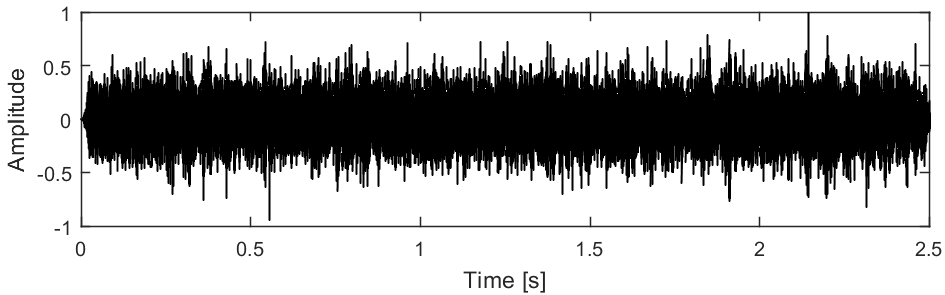
\includegraphics[width=\textwidth]{wykresy/chapter_application/semi_blind/sygnal_bez_impulsow_filtr.png}
        \label{fig:chapter7/semi_blind/time_zdrowy_filtr}
    \end{subfigure}

    \begin{subfigure}[b]{0.8\textwidth}
        \centering
        \captionsetup{skip=0.01pt}
        \caption{}
        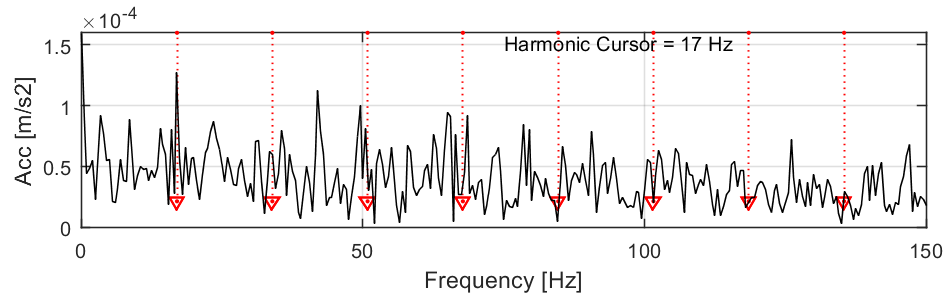
\includegraphics[width=\textwidth]{wykresy/chapter_application/semi_blind/widmo_obwiedni_sygnal_bez_impulsow_filtr.png}
        \label{fig:chapter7/semi_blind/obwiednia_zdrowy_filtr}
    \end{subfigure}
    \caption{Time plot (a) and envelope spectrum (b) of the extracted cyclic normalized signal component with bearing jitter effect.}
\end{figure}
\section{Real data analysis}
\subsection{Cyclic sources extraction from complex multiple-component vibration signal via periodically time varying filter}
\label{sec:chapter7/semi_blind/schemat_przekladniaapplication_real}
Once the performance of the algorithm was tested on the simulated data, it can be applied to the real signal. In this section results of the methodology application to the vibration data recorded on the belt conveyor gearbox are presented. Analyzed machine is located in the underground copper ore mine, thus it works in harsh environment. Kinematic scheme of the analyzed gearbox is presented in Fig.~\ref{fig:chapter7/semi_blind/schemat_przekladnia}. The gearbox is equipped with two stages - the first bevel pair is followed by the spur pair. The electric engine rotor speed is around 996 rpm, thus the first shaft rotates with the frequency close to 16.61~Hz. Variability of the rotational speed does not exceed $\pm1.5$ rpm. The rotational frequency of the second shaft is 4.2~Hz, since the first stage ratio is equal to 91:23. The vibration signal was acquired on three different spots of the machine (Fig.~\ref{fig:chapter7/semi_blind/pomiar}). Moreover, the rotational speed was also acquired in order to ensure that it is almost constant during the experiment. Sampling frequency is 17066~Hz and the signal duration is equal to 5 seconds. The exemplary local fault in the gear is illustrated in Fig.~\ref{fig:chapter7/semi_blind/damage}.
%
\begin{figure}[ht!]
\centering
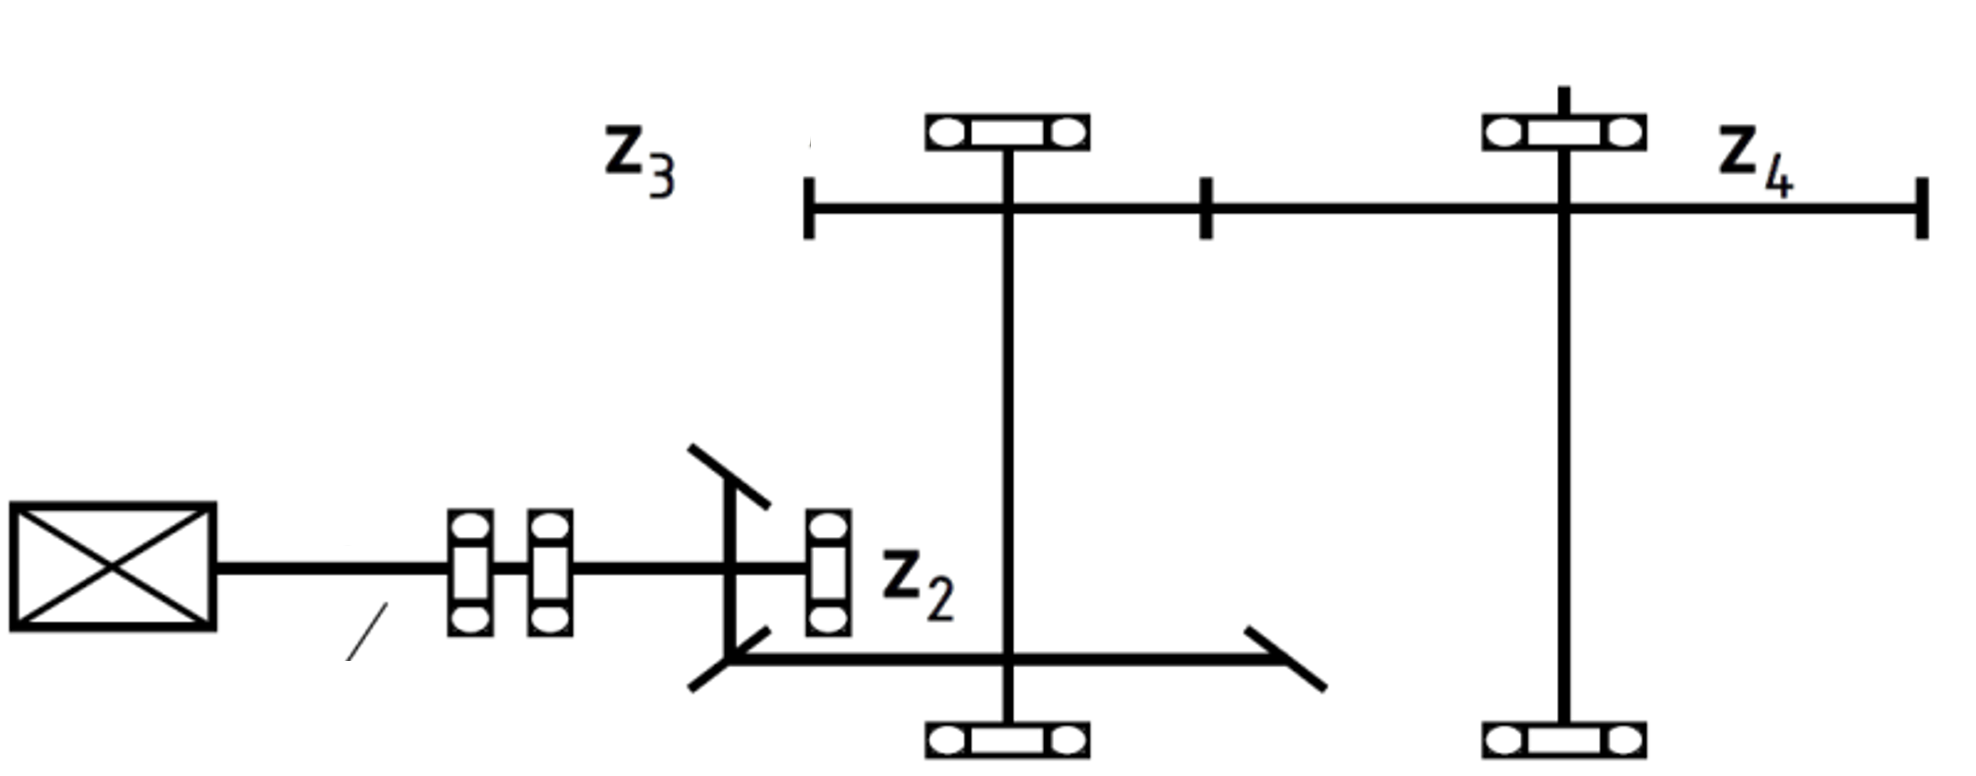
\includegraphics[width=1\textwidth]{wykresy/chapter_application/semi_blind/schemat_przekladnia}
\caption{Kinematic scheme of the analyzed gearbox. The number of teeth in each stage: $z_1=23$, $z_2=91$, $z_3=44$ and $z_4=155$.}
\label{fig:chapter7/semi_blind/schemat_przekladnia}
\end{figure}
%
\begin{figure}[!ht]
    \centering
    \begin{subfigure}[b]{0.49\textwidth}
        \centering
        \captionsetup{skip=0.01pt}
        \caption{}
        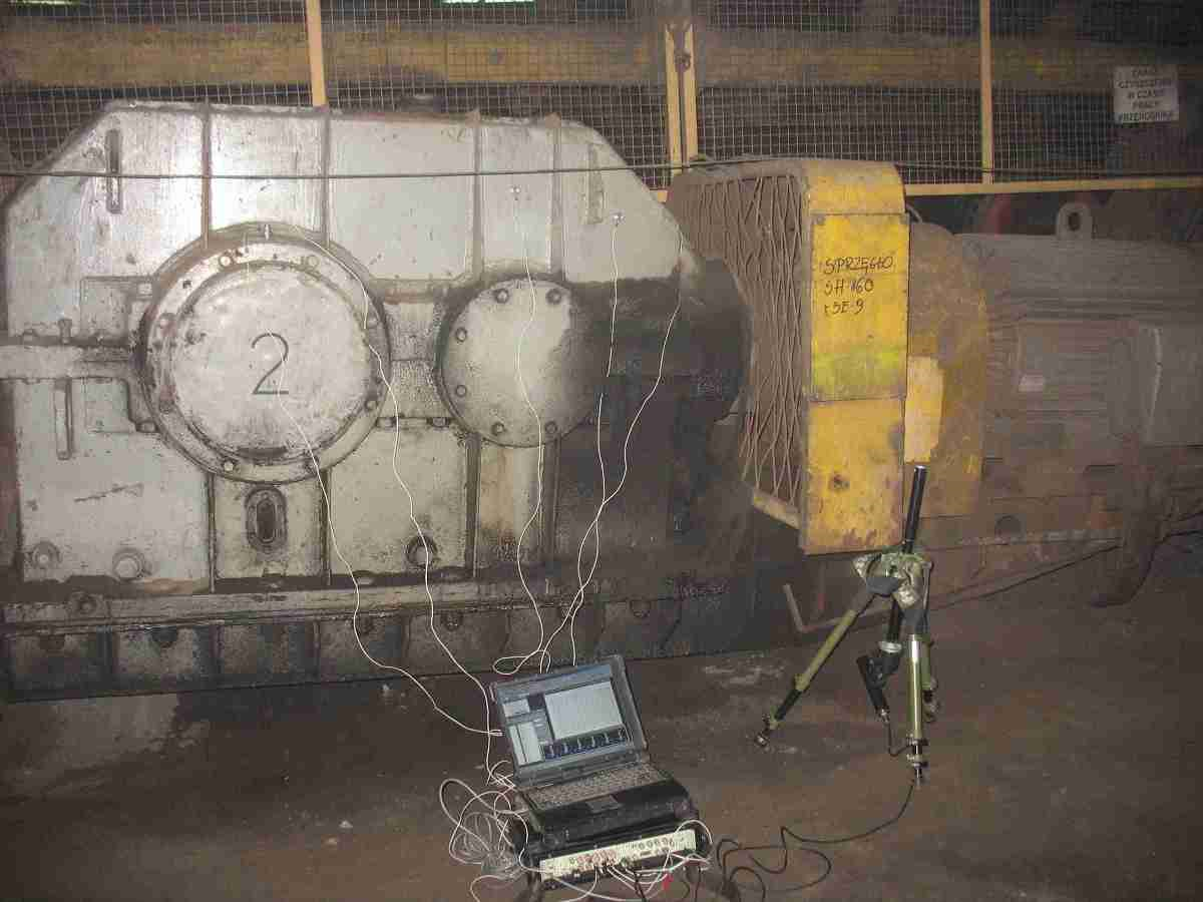
\includegraphics[width=\textwidth]{wykresy/chapter_application/semi_blind/czujniki}
        \label{fig:chapter7/semi_blind/pomiar}
    \end{subfigure}
    %\hfill
    \begin{subfigure}[b]{0.49\textwidth}
        \centering
        \captionsetup{skip=0.01pt}
        \caption{}
        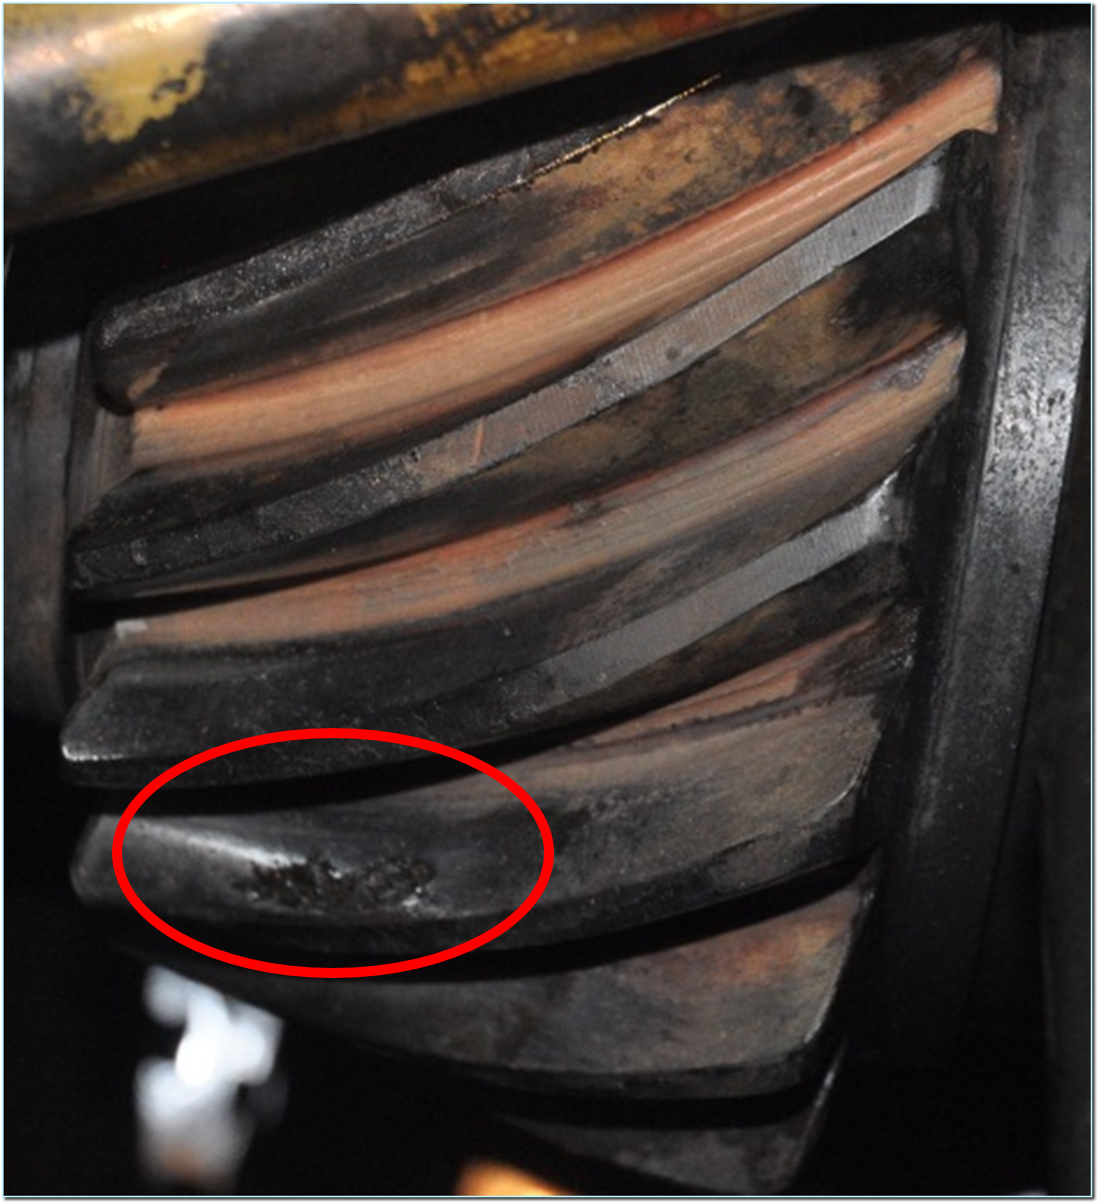
\includegraphics[width=\textwidth]{wykresy/chapter_application/semi_blind/damage}
        \label{fig:chapter7/semi_blind/damage}
    \end{subfigure}    
    \caption{The data acquisition system during the experiment (a) and exemplary local damage in the gear (b).}
\end{figure}
%
\\
The signal reveals two faults in the machine related to the rotating speed of first and second shaft. The signal in time domain is presented in Fig.~\ref{fig:chapter7/semi_blind/time_L212}. The raw spectrogram (Fig.~\ref{fig:chapter7/semi_blind/spectrogram_L212}) reveals some frequency bands with high energy. These are related to gear mesh frequencies (379.5~Hz and 183.3~Hz for first and second stage, respectively) and their harmonics. There are lots of  wideband excitations, although it is difficult to state if they are related to any cyclic pattern. Thus, it is worth to apply the proposed source extraction algorithm.
\begin{figure}
    \centering
    \vspace{-1\baselineskip}
    \begin{subfigure}[b]{0.8\textwidth}
        \centering
        \captionsetup{skip=0.01pt}
        \caption{}
        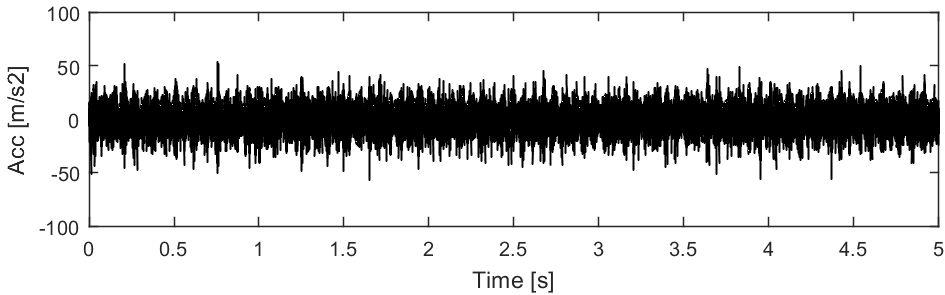
\includegraphics[width=\textwidth]{wykresy/chapter_application/semi_blind/sygnalL212.png}
        \label{fig:chapter7/semi_blind/time_L212}
    \end{subfigure}
     \vspace{-1\baselineskip}
    \begin{subfigure}[b]{0.8\textwidth}
        \centering
        \captionsetup{skip=0.01pt}
        \caption{}
        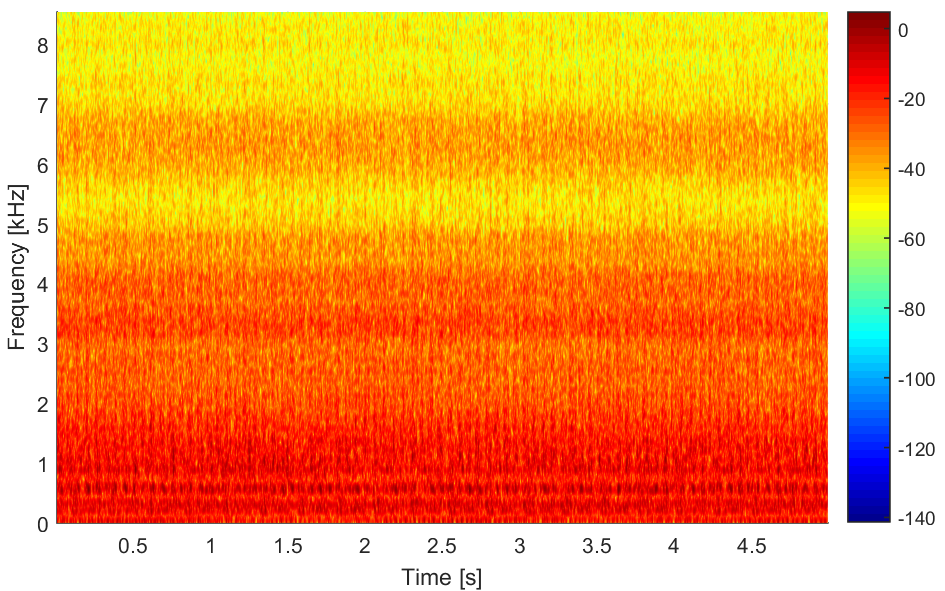
\includegraphics[width=\textwidth]{wykresy/chapter_application/semi_blind/spectrogramL212.png}
        \label{fig:chapter7/semi_blind/spectrogram_L212}
    \end{subfigure}
    \begin{subfigure}[b]{0.8\textwidth}
        \centering
        \captionsetup{skip=0.01pt}
        \caption{}
        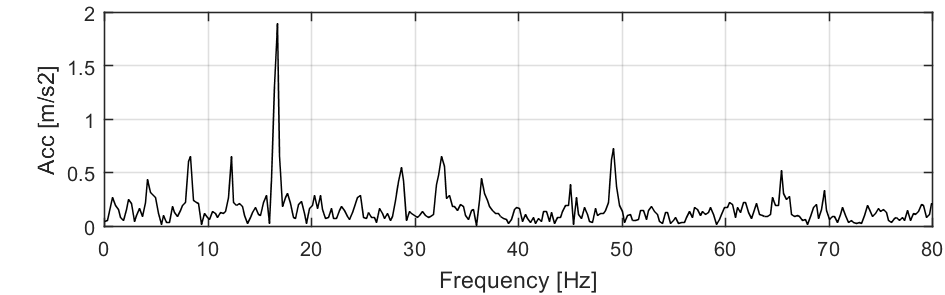
\includegraphics[width=\textwidth]{wykresy/chapter_application/semi_blind/widmo_obwiedniL212.png}
        \label{fig:chapter7/semi_blind/obwiednia_L212}
    \end{subfigure}
    \caption{Time plot (a), spectrogram (b) and envelope spectrum (c) of the real signal recorded on the belt conveyor's gearbox. The spectrogram parameters are as follows: $N_w=250$, $Ov=96\%$.}\label{fig:chapter7/semi_blind/time-plot_L212}
\end{figure}
\\
As in the simulated data case, two fault frequencies are considered, namely, 4.2~Hz and 16.61~Hz. Score maps for two fault frequencies are presented in Figs.~\ref{fig:chapter7/semi_blind/wagi_L212_4} and~\ref{fig:chapter7/semi_blind/wagi_L212_16}. Some barely visible periodic patterns might be noticed in both figures. The pattern related to 4.2~Hz is located in carrier frequency band lower than 1000~Hz. The second pattern reveals in almost every frequency band, including the lowest frequencies. Thus, this signal is more challenging than the simulated data, since in a single frequency band two periodic modulations occur and one of them reveals in a relatively narrow frequency band. Moreover, two different phases can be detected in case of 4.2~Hz modulation frequency (see arrows in Fig.~\ref{fig:chapter7/semi_blind/wagi_L212_4}), i.e. two different components with modulation frequency close to 4.2~Hz can be noticed. The related carrier frequencies are 0-400~Hz and 500-700~Hz, respectively. Such phenomenon might be caused by two different local faults occurring on the second shaft, for instance one on the bevel gear and second on the spur gear. Therefore, carrier frequency bands might be different due to different transmission path.
\begin{figure}[!ht]
    \centering
    \begin{subfigure}[b]{0.49\textwidth}
        \centering
        \captionsetup{skip=0.01pt}
        \caption{}
        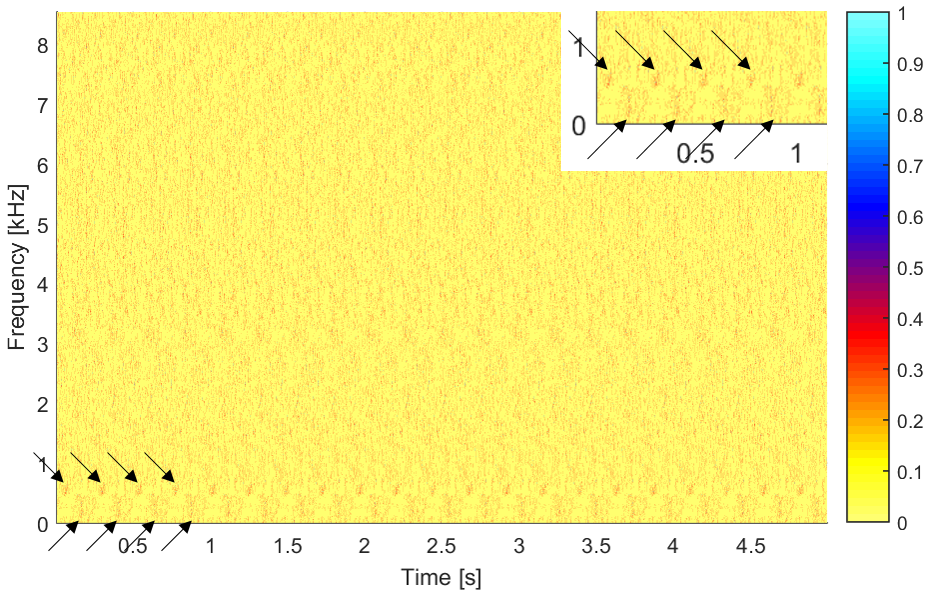
\includegraphics[width=\textwidth]{wykresy/chapter_application/semi_blind/wagiL212_4.png}
        \label{fig:chapter7/semi_blind/wagi_L212_4}
    \end{subfigure}
     \vspace{-1\baselineskip}
    \begin{subfigure}[b]{0.49\textwidth}
        \centering
        \captionsetup{skip=0.01pt}
        \caption{}
        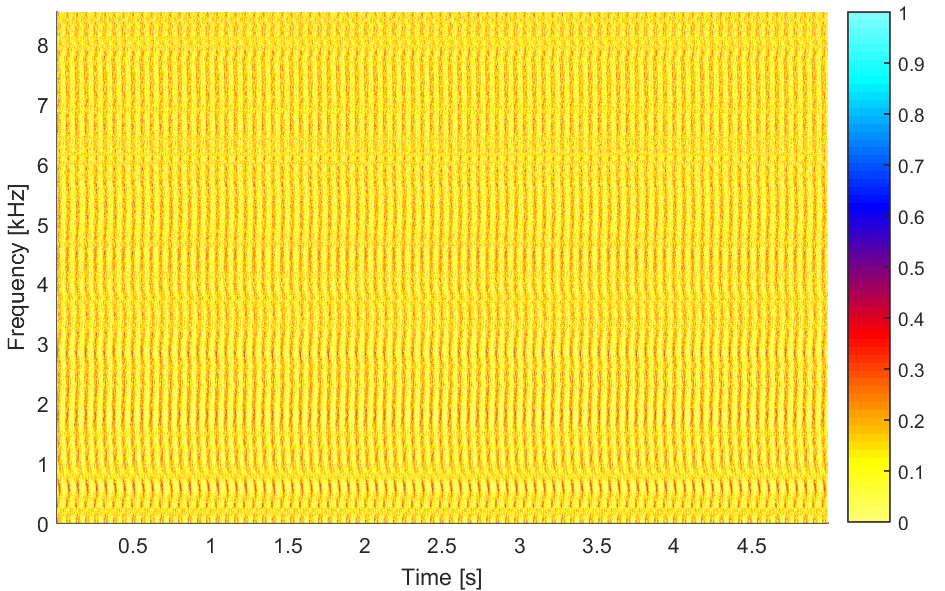
\includegraphics[width=\textwidth]{wykresy/chapter_application/semi_blind/wagiL212_16.png}
        \label{fig:chapter7/semi_blind/wagi_L212_16}
    \end{subfigure}
     \vspace{-1\baselineskip}
    \begin{subfigure}[b]{0.49\textwidth}
        \centering
        \captionsetup{skip=0.01pt}
        \caption{}
        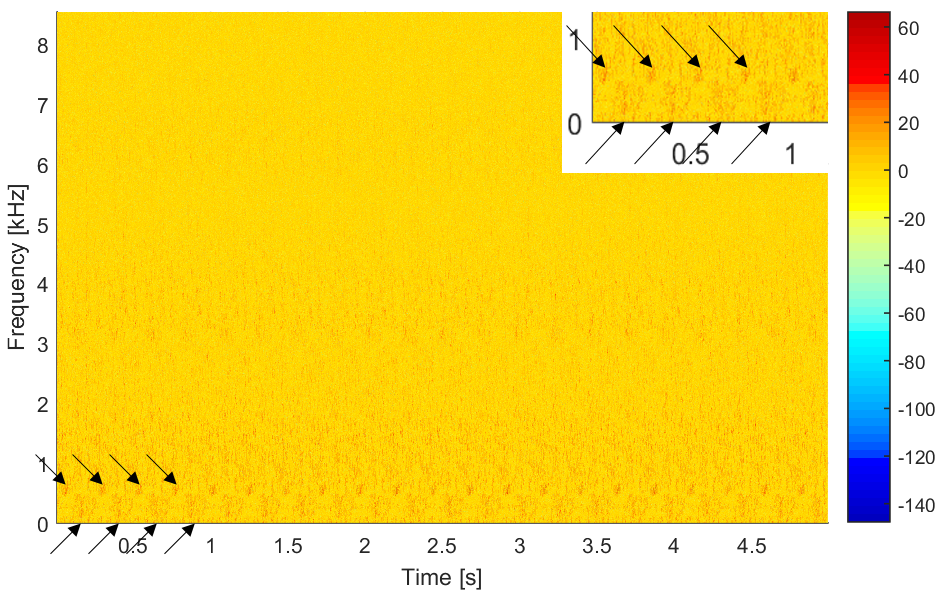
\includegraphics[width=\textwidth]{wykresy/chapter_application/semi_blind/mapkaL212_log_4.png}
        \label{fig:chapter7/semi_blind/mapka_L212_4}
    \end{subfigure}
    %\hfill
    \begin{subfigure}[b]{0.49\textwidth}
        \centering
        \captionsetup{skip=0.01pt}
        \caption{}
        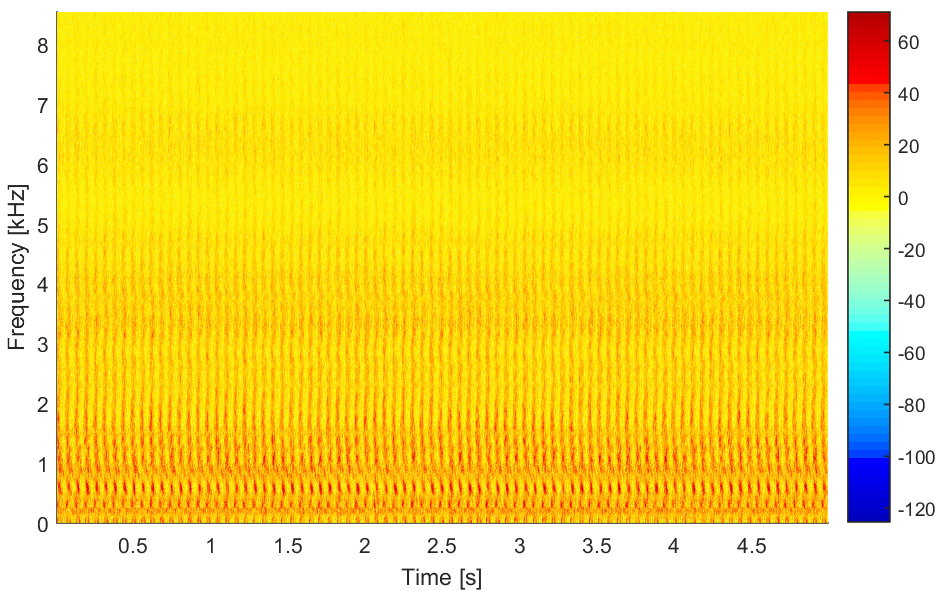
\includegraphics[width=\textwidth]{wykresy/chapter_application/semi_blind/mapkaL212_log_16.png}
        \label{fig:chapter7/semi_blind/mapka_L212_16}
    \end{subfigure}
    \caption{Score matrices for fault frequency 4.2~Hz (a) and 16.61~Hz (b). The weighted spectrograms in the log scale for fault frequency 4.2~Hz (c) and 16.61~Hz (d). }\label{fig:chapter7/semi_blind/score_real}
%
% zoomed maps
    \centering
    \begin{subfigure}[b]{0.49\textwidth}
        \centering
        \captionsetup{skip=0.01pt}
        \caption{}
        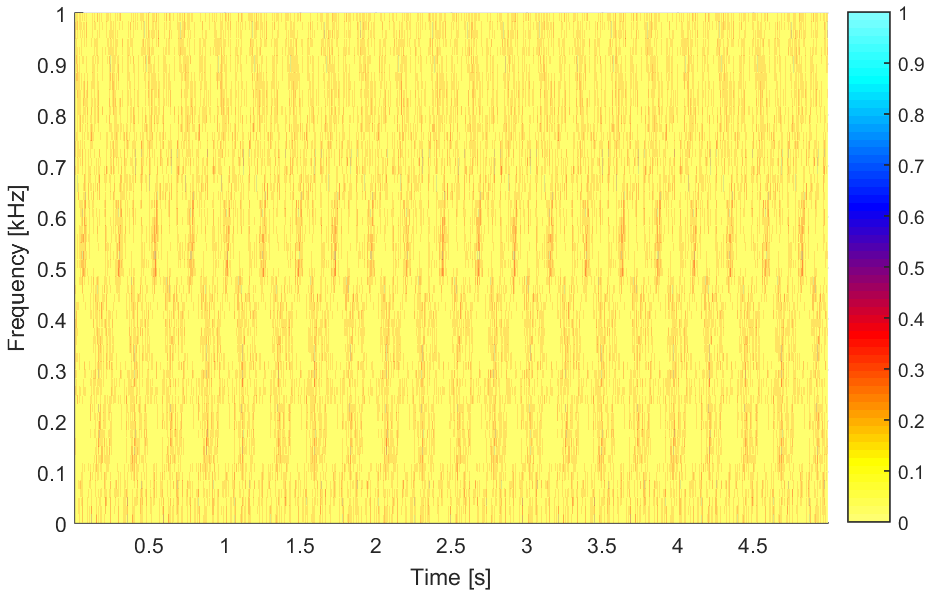
\includegraphics[width=\textwidth]{wykresy/chapter_application/semi_blind/wagiL212_4_zoom.png}
    \end{subfigure}
    %\hfill
    \begin{subfigure}[b]{0.49\textwidth}
        \centering
        \captionsetup{skip=0.01pt}
        \caption{}
        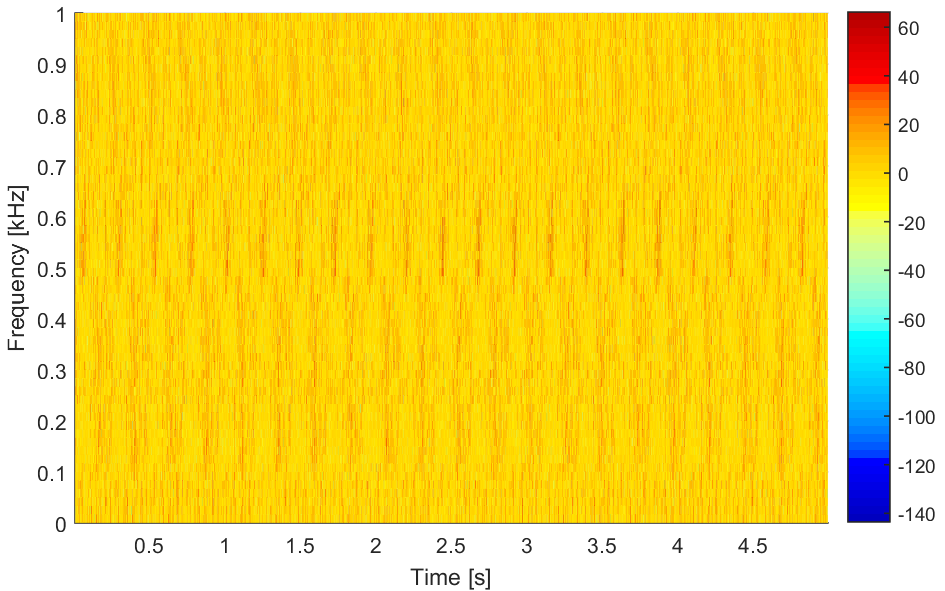
\includegraphics[width=\textwidth]{wykresy/chapter_application/semi_blind/mapkaL212_log_4_zoom.png}
    \end{subfigure}    
    \caption{The zoomed score matrix for fault frequency 4.2~Hz (a) and zoomed weighted spectrogram in the log scale for fault frequency 4.2~Hz (b).}\label{fig:chapter7/semi_blind/score_zoom}
\end{figure}
%
% widma obwiedni
\begin{figure}[!ht]
    \centering
    \begin{subfigure}[b]{0.49\textwidth}
        \centering
        \captionsetup{skip=0.01pt}
        \caption{}
        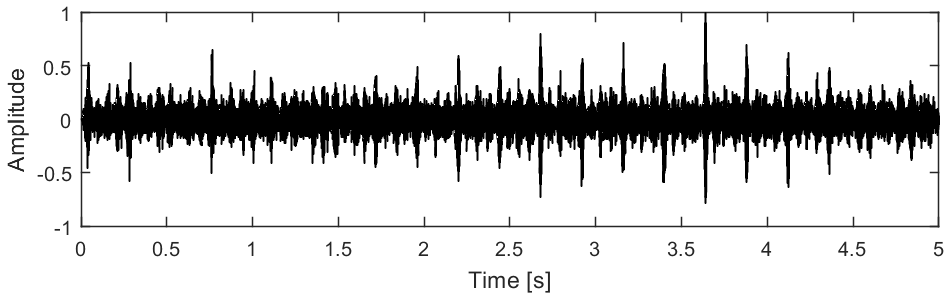
\includegraphics[width=\textwidth]{wykresy/chapter_application/semi_blind/sygnalL212_4.png}
        \label{fig:chapter7/semi_blind/ext_comp_L212_4}
    \end{subfigure}
     \vspace{-1\baselineskip}
    \begin{subfigure}[b]{0.49\textwidth}
        \centering
        \captionsetup{skip=0.01pt}
        \caption{}
        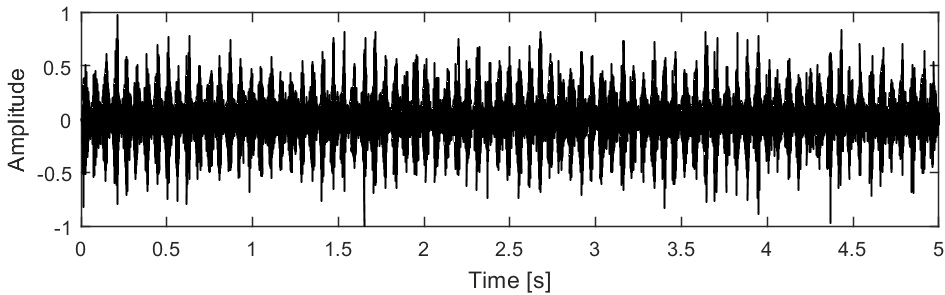
\includegraphics[width=\textwidth]{wykresy/chapter_application/semi_blind/sygnalL212_16.png}
        \label{fig:chapter7/semi_blind/ext_comp_L212_16}
    \end{subfigure}
     \vspace{-1\baselineskip}
    \begin{subfigure}[b]{0.49\textwidth}
        \centering
        \captionsetup{skip=0.01pt}
        \caption{}
        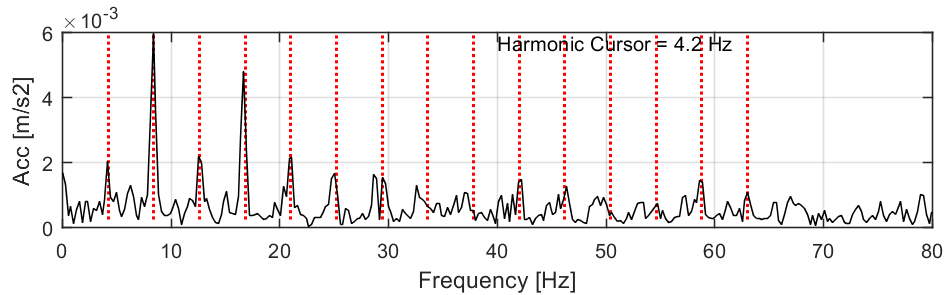
\includegraphics[width=\textwidth]{wykresy/chapter_application/semi_blind/widmo_obwiedniL212_4.png}
        \label{fig:chapter7/semi_blind/ext_widmo_obwiedni_L212_4}
    \end{subfigure}
        \begin{subfigure}[b]{0.49\textwidth}
        \centering
        \captionsetup{skip=0.01pt}
        \caption{}
        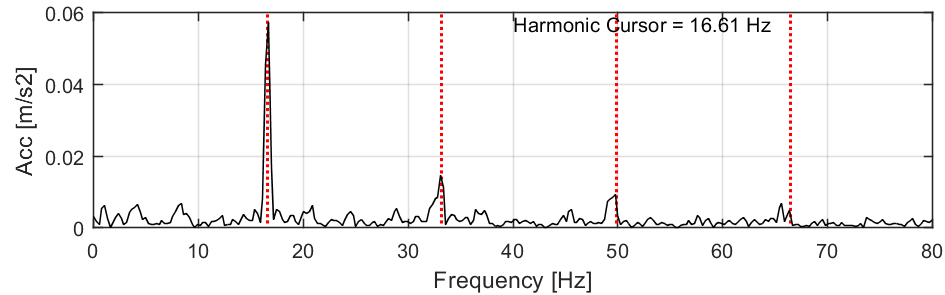
\includegraphics[width=\textwidth]{wykresy/chapter_application/semi_blind/widmo_obwiedniL212_16.png}
        \label{fig:chapter7/semi_blind/ext_widmo_obwiedni_L212_16}
    \end{subfigure}
    \vspace{\baselineskip}
    \caption{The normalized extracted signals from weighted spectrograms for fault frequency 4.2~Hz (a) and 16.61~Hz (b). The envelope spectra of the extracted signals for fault frequency 4.2~Hz (c) and 16.61~Hz (d). }\label{fig:chapter7/semi_blind/signal_ext}
\end{figure} 


Weighted spectrograms are illustrated in Figs.~\ref{fig:chapter7/semi_blind/mapka_L212_4} and~\ref{fig:chapter7/semi_blind/mapka_L212_16}. One can observe that the level of background noise is relatively small and the periodic excitations are with relatively high amplitudes.  In order to transform weighted spectrogram to time domain the inverse short-time Fourier transform can be applied. Therefore, the cyclic component is extracted. The results are presented in Figs.~\ref{fig:chapter7/semi_blind/ext_comp_L212_4} and~\ref{fig:chapter7/semi_blind/ext_comp_L212_16}. Two different in phase pulse trains with modulation frequency 4.2~Hz might not be clearly visible, since the corresponding score values are relatively low. Excitations related to the second fault are clearly visible. Given the extracted components, envelope analysis might be performed in order to check periodicity of the extracted signals. According to Figs.~\ref{fig:chapter7/semi_blind/ext_widmo_obwiedni_L212_4} more than 10 harmonics of 4.2~Hz might be noticed which corresponds to impulsive character of the source signal. It is worth to notice that in the carrier frequency band 0-1000~Hz both modulation frequencies are revealed. Moreover, filter coefficients related to 16.61~Hz are the highest in the band from 0~Hz up to 2000~Hz, among both filter characteristics - it ensures that there are significant local maxima with related range. Nevertheless, the signal filtered using the weighted spectrogram calculated for 4.2~Hz does not contain significant amplitude modulations of 16.61~Hz. Hence, even such sources might be separated and damage detection can be performed with introduced novel method.